\section{Preface}
\textit{The following chapter develops a model called The Elastic Neighbourhood which incorporates an understanding of competition into the seminal Elastic Net model. The research aim was to develop a heuristic which integrated modern scientific understanding of topographic map development with the Elastic Net heuristic. The focus of this chapter will be on the algorithms development which follows directly from the model proposed in the previous chapter and to demonstrate its efficiency at solving large scale instances of the problem competitively against the best current heuristics: EAX-GA and LHK. The model is also examined as a feature map generator and it is shown to generate feature maps with less underlying retinotopic distortion than the Elastic Net.}

\section{Introduction \label{section:elasticintro}}
Chapter \ref{chapter:distributed} developed a parallelised model of topographic development based on an energy minimisation approach whereby developmental each mechanism can be incorporated into a sum of linearly independent energies. The result was a computationally efficient and interpretable model that reproduced available biological data; improving on existing models in runtime and predictive power. The energy equations resemble an abstract model of neural development and a Travelling Salesman heuristic: the Elastic Net \cite{Durbin1987-ki}. The Elastic Net was born out of an early model of topographic development, the Tea-Trade activity model \cite{Willshaw1976-ew}, and the results of the previous chapter therefore suggest that the Elastic Net methodology can be improved by incorporating analogous mechanisms of biological topographic development. The Travelling Salesman Problem (TSP) will be introduced before detailing the Elastic Net and applications.
\paragraph{The Travelling Salesman Problem}
The Travelling Salesman is an open NP-complete problem in computer science which is simply stated as: given a collection of nodes with possibly asymmetric distances between them, find the shortest path that visits each node once before returning to the origin \cite{Applegate2007-nz}. This is shown in Figure \ref{fig:TSPexample}. A valuable property of NP-complete problems is the existence of a polynomial-time mapping from any problem into the other, thus solving a single NP-complete problem efficiently yields benefits in analogous problems \cite{Garey1990-th}. The TSP is used commonly used to benchmark optimisation algorithms and many more scientifically grounded problems are mathematically equivalent or can be distilled to a version of the TSP. Such problems include vehicle routing, protein folding, topographic organisation, and neural wire minimisation \cite{Ball2002-hf, Guo2007-ub, PaoloToth2002Tvrp, Durbin1990-tn}. The generality of the problem has led a wealth of exact and heuristic solvers.
\begin{figure}
	\begin{subfigure}{0.5\linewidth}
		\includegraphics[width = \textwidth]{images/introduction/tourscatter}
		\caption{} 
	\end{subfigure}
	~
	\begin{subfigure}{0.5\linewidth}
		\includegraphics[width = \textwidth]{images/introduction/tourvalid}
		\caption{} 
	\end{subfigure}
	\def\c{A description of the Travelling Salesman Problem. }
	\caption[\c]{A series of nodes scattered uniformly in the unit square is shown in the left panel (a) while a valid tour passing through each of these nodes once before returning to the initial node is shown in the right panel (b). There are n! such tours and while this example does not exhibit a tour crossing they are ostensibly possible. Due to the metric triangle inequality any tour with a crossing can be improved and they are thus provably sub-optimal. Figure reproduced from Chapter \ref{chapter:review} \label{fig:TSPexample}}
\end{figure}
The computational complexity has a minimal upper bound of $\mathcal{O}(n^2 2^n)$ which involve branch-and-bound methodologies and have been largely incorporated into the well optimised Concorde TSP solver \cite{Applegate2007-nz}. The super-polynomial runtime renders exact solutions nearly impossible to generate for even modest tours: tours from the Art Dataset, such as the Mona Lisa, have over $100,000$ nodes and require a large amount of computational runtime for very modest improvements of bounds and the exact solution has remained an open question for the last decade \cite{ArtTSP}. As a result, most applications use heuristics which deliver acceptable performance, often under 10\% of the true minima, at a much cheaper computational cost: the accuracy-speed trade-off is of utmost importance in these problems. The two prevailing heuristics are the Lin–Kernighan heuristic (LKH) and a genetic algorithm which mutates the Edge-Assembly Crossover (EAX-GA) \cite{Helsgaun2009-dl, Lin1973-pt,  Nagata2013-we, Honda2013-ri}. EAX-GA comes from the broader class of biologically inspired heuristics which have proved to be a fruitful domain for heuristic generation; for a review see Halim et. al. (2019) \cite{Halim2019-ch}. A recent review of TSP heuristics offers a blueprint to formally compare heuristics involving the computational wall-time and form of the data and, focusing on LKH and EAX-GA, found that in most cases EAX-GA was the faster and more accurate algorithm \cite{McMenemy2019-rl}. While their approach focused on solving the problem exactly and adding a time penalty if the algorithm failed to converge the idea can be extended to formalising the cost-performance trade off for a particular problem.
 
\paragraph{The Elastic Net}
The model is an energy minimisation model which deforms a net of elastic beads, where neighbours are connected elastically by spring forces, to a set of nodes (or cities) which provide attractive forces to each of the beads. Supposing that there are $N$ nodes and $M$ beads and letting $X = \{\vec{x}_i : i = 1, ..., N \}$ and $Y = \{\vec{y}_i : i = 1, ..., M \}$ the energy of a given bead configuration is given by a functional parametrised by $\alpha, \beta, K$:
\begin{equation}
E[Y|X; \alpha, \beta, K] = -\alpha \sum_{i = 1}^{M} \log \left( \sum_{j=1}^N \exp\left ( \frac{- \lVert \vec{x}_i - \vec{y}_j \rVert^2 }{ 2 K^2 }  \right) \right) + \beta \sum_{j=1}^{N} \lVert \vec{y}_j - \vec{y}_{j-1} \rVert^2,
\end{equation}
In the limiting case of $K\rightarrow0$ the attractive energy provided in the first term is only significant in a small radius around each node while the tension term dominates in all other areas. The local minima of this functional in this limit are therefore straight line geodesics corresponding to the tension term that travel between each of the cities. Thus, these minima correspond to valid tours of the TSP. The functional can be minimised by gradient descent to find a local minima $K$; see Section \ref{sec:minimisation}. The gradient is calculated as:
\begin{equation}
\frac{\partial \vec{y}_j(t)}{\partial t}  = \beta K \left(\vec{y}_{j-1} - 2 \vec{y}_j + \vec{y}_{j+1}  \right) + \alpha \sum_{i = 1}^M (\vec{x}_i - \vec{y}_j) W(\vec{x}_i, \vec{y}_j, K(t); Y) + \gamma \sum_{i = 1}^M (\vec{y}_i - \vec{y}_j) W(\vec{y}_i, \vec{y}_j, K(t); Y),
\end{equation}
where $W(\vec{z}_i, \vec{y}_i, K; Y) = \exp(- \lVert \vec{x}_i - \vec{y}_j \rVert^2 / (2 K^2)) / \sum_{j = 1}^N \exp(- \lVert \vec{z}_i - \vec{y}_j \rVert^2 / (2 K^2))$. This rule is applied 25 times for each $K$ after which $K$ is reduced by the mapping $K\leftarrow0.99K$. When $K$ has reached a sufficiently low value the procedure is terminated.
\paragraph{Generalised Elastic Nets \label{sec:generalisedEN}}
The Elastic Net was motivated primarily as a TSP-heuristic derived from principles of neural activity \cite{Willshaw1976-ew}. The Laplacian operator with circular boundary conditions was implemented to offer a minimisation target for tour length as well as enforcing continuity conditions with the index of the bead thus defining valid tours. This mechanism can be seen as preserving topography from index space to neural space: neighbouring indexes remain neighbouring in their neural position. This observation means that it can be naturally extended to a formal model of topography by defining the net not on a line by a grid of indexes corresponding to some neural space and allowing the Laplacian operator be applied to all neighbours of a cell $j$ on this grid:
\begin{equation}
E_\text{neigh}[Y; \beta] = \beta \sum_{j=1}^{M}\sum_{k=\in\text{neigh}(j)} \lVert \vec{y}_k - \vec{y}_{j} \rVert.
\end{equation}
The vector $\vec{y} = (y_1, y_2)$ has been constructed to correspond to the receptive field of a position in space and this term tends to aggregate points which are neighbouring on the cortical grid while the activity term pulls them to what can be considered as presentations or samples of receptive field space. This can be further extended to a topological with $P$ features by letting $\vec{y} = (y_1,...,y_P)$ where each coordinate represents a feature: position in space, orientation selectivity, left-right eye input etc. In this fashion the Elastic Net has been used to account for orientation selectivity, retinotopy, and ocular dominance \cite{Goodhill2000-on, Goodhill1994-dn, Goodhill2000-vp, Goodhill1990-dr, Durbin1990-tn}. The model was also used to suggest that the brain uses developmental principles to minimise the amount of neural wiring required to encode its computational feature space concordant with the wire minimisation hypothesis \cite{Durbin1990-tn, Swindale1992-de, Swindale2001-gh, Koulakov2001-je}. Finally, the neighbourhood approach can be naturally generalised to an arbitrary set of neighbours, not just nearby neighbours in index (cortical) space. These functions may be thought of \textit{stencils} and for a general discussion about them see Carreira-Perpi{\~n}{\'a}n and Goodhill (2011) \cite{Carreira-Perpinan2011-aa}.
\paragraph{Improvements}
Development of the Elastic Net has focused primarily on parameter selection with analysis determining optimal rules of thumb for setting the $\alpha/\beta$ ratio and discussion about the limiting aspects of this and how they may be compensated with additional parameter manipulation such as the node-bead ratio \cite{Simmen1991-hm, Durbin1989-gs}. A variation of the Elastic Net was proposed to give substantial computational performance reducing the amount of information considered at each step with minimal performance loss \cite{Boeres1992-fo, Burr1988-fg}.

Chapter \ref{chapter:distributed} suggests that a more fundamental approach can be used to improve the performance of the Elastic Neighbourhood: adding the developmental role of competition. The Elastic Net methodology is expected to offer a more convincing explanation of topological feature maps by incorporating this mechanism. The methodology is also expected to see technical improvements in runtime by adopting the GPU based architectures used in the previous chapter used in conjunction with the ADAM optimiser \cite{kingma2017adam}. These improvements shall be collectively referred to as the Elastic Neighbourhood and will be detailed in the following section.
\section{Method}
The problem is set up in the same manner as the EN: there exists a series of nodes indexed by $i \in \{1, ..., M\}$ and of beads indexed by $j \in \{1, ..., N\}$. Each node is defined by its coordinate position $i \mapsto \vec{x}_i$ and each bead is defined by its coordinate position at a given time $j \mapsto \vec{y}_j(t)$. The space is equipped with a metric $d:  \mathbb{R} \times  \mathbb{R} \rightarrow \mathbb{R}$ forcing the problem to be the symmetric TSP, and the node coordinates are scaled so that they lie within the unit box centred around the origin: $\{  {\lVert \vec{x}_i \rVert}_{\infty}  \leq 1 \quad \forall \quad 1\leq i \leq M \} $ where the $\lVert.\rVert_\infty$ denotes the infinity norm. 
\subsection{Energy Functional} \label{section:neighbourhoodenergyfunctional}
The Elastic Net mechanisms each have relationships with existing topographic map developmental mechanisms. Section \ref{section:elasticintro} demonstrated how the term associated with $\beta$ may be thought of as topographic when extended to receptive field space and allowing the index terms to encode positional information. Note that this correspond to a Type II lock-and-key mechanism employed by chemotaxis; see Section \ref{sec:models}. The activity energy is slightly more involved: in biological systems there are waves of correlation activity which over time decrease in the area which they span in the pre-synaptic and post-synaptic targets ultimately leading to a greater refinement of topography \cite{Stafford2009, Seabrook2017-fa}. To capture this each node is imbued with the ability to attract over some region in the post-synaptic target and this region is progressively decreased over time. Therefore, the beads (afferents) are allowed to be mobile in the exploration of the target but must eventually converge to a singular location reflecting the motility afferents enjoy in early development and subsequent refinement into precise zones. This information is incorporated by saying that the interaction energy a node $i$ exerts on a bead $j$ is proportional to $\exp\left ( - \lVert \vec{x}_i - \vec{y}_j \rVert^2 / (2 K^2)  \right)$. Therefore, letting $K\rightarrow 0$ implies the domain of influence shrinks. A salient point made in the original work was that the effect of each node should be normalised i.e. each node should contribute an equal amount when its energy interactions with each bead are calculated. This can be achieved by employing an attention mechanism via the natural logarithm for a total activity energy contribution of:
\begin{equation}\label{eq:actneighbourenergy}
E_\text{act}[Y; \alpha, K]  = -\alpha \sum_{i = 1}^{M} \log \left( \sum_{j=1}^N \exp\left ( \frac{- \lVert \vec{x}_i - \vec{y}_j \rVert^2 }{ 2 K^2 }  \right) \right).
\end{equation} 
A particular challenge to the EN is that all tours are local minima which can be seen by the fact that while the diffusion operator enforces local continuity it does not prevent beads multiple steps away in the path from crossing over: there is no interaction of beads outside of their pre-defined neighbours. This is improved by including a third key component of topographic mapping: competition. Each bead is now allowed to interact with all other beads to try and establish local dominance over a region corresponding to the competition of afferents in biological systems for physical space and metabolic resources. As for activity, each afferent is assumed to have a competitive region which becomes more concentrated as its arbour refines over time resulting in beads $j$ and $k$ contributing an energy proportional to $\exp\left ( - \lVert \vec{y}_i - \vec{y}_j \rVert^2 / (2 U^2)  \right)$. For simplicity, assuming $U = K$ implies the competition falls in lock-step with the activity contribution, justified by the fact that an afferents arbour, the underlying object of interest, decreases at this rate. Assuming that each bead has the same competitive potential necessitates the attention mechanism as before resulting in an energy contribution of: 
\begin{equation} \label{eq:compneighbourenergy}
E_\text{comp}[Y; \gamma, K]  = \gamma \sum_{j = 1}^{N} \log \left( \sum_{k=1}^N \exp\left ( \frac{- \lVert \vec{y}_j - \vec{y}_k \rVert^2 }{ 2 K^2 }  \right) \right).
\end{equation}
This energy contribution allows for the interaction of all beads with each other in a given local neighbourhood and is thus called: \textit{the Elastic Neighbourhood}. The competitive energy has the advantage that when a portion of the tour attempts to form a crossover it induces a large spike in the energy and thus makes such cross-overs cost prohibitive. This is advantageous for a gradient descent algorithm minimisation scheme because it means that the initial curve and the final curve defining the tour will be homotopically equivalent (provided a sufficiently small step size) and the solution to a TSP must equivalent to that of a circle. The addition of this term thereby precludes many tours from being energy minima and restricts the search to a known subset of potential solutions \cite{Applegate2007-nz}. The total energy function is defined by:
\begin{equation} \label{eq:totalneighbourenergy}
\begin{split}
E[Y; \alpha, \beta, \gamma, K] &= -\alpha \sum_{i = 1}^{M} \log \left( \sum_{j=1}^N \exp\left ( \frac{- \lVert \vec{x}_i - \vec{y}_j \rVert^2 }{ 2 K^2 }  \right) \right) + \beta \sum_{j=1}^{N} \lVert \vec{y}_j - \vec{y}_{j-1} \rVert^2  \\ 
& \quad + \gamma \sum_{j = 1}^{N} \log \left( \sum_{k=1}^N \exp\left ( \frac{- \lVert \vec{y}_j - \vec{y}_k \rVert^2 }{ 2 K^2 }  \right) \right).
\end{split}
\end{equation}
In the limit $K \rightarrow 0$ the local minima define valid tours as in the EN. This can be seen as a result of the linearity of combining each mechanism and the competition mechanism becoming negligible in the low $K$ regime: there is a $K$ for which the beads are sufficiently far away from each other that they do not interact.
\subsection{Minimisation}
As alluded to in Section \ref{section:neighbourhoodenergyfunctional} a gradient descent based scheme is used to minimise the energy functional. ADAM is an accelerated gradient descent algorithm that has found much success in the field of machine learning and is used instead of vanilla gradient descent, as in the original algorithm. The ADAM operator updates a positional value, in this case $\vec{y}_j$, by a combination of the gradient and the previous update; for details see \cite{kingma2017adam}. The scaled gradient of $\vec{y}_j$ at time $t$ is calculated as the functional derivative of $E[Y]$ with respect to $\vec{y}_j(t)$:
\begin{equation}
\frac{ \partial \vec{y}_j(t)}{\partial t}= -K(t) \frac{\delta E[Y]}{\delta \vec{y}_j(t)},
\end{equation}
which after combining all individual energy terms equation \ref{eq:totalneighbourenergy} is calculated as:
\begin{equation}
\frac{\partial \vec{y}_j(t)}{\partial t} = \beta K \left(\vec{y}_{j-1} - 2 \vec{y}_j + \vec{y}_{j+1}  \right) + \alpha \sum_{i = 1}^M (\vec{x}_i - \vec{y}_j) W(\vec{x}_i, \vec{y}_j, K(t); Y) + \gamma \sum_{i = 1}^M (\vec{y}_i - \vec{y}_j) W(\vec{y}_i, \vec{y}_j, K(t); Y),
\end{equation}
where $W(\vec{z}_i, \vec{y}_i, K; Y) = \exp(- \lVert \vec{x}_i - \vec{y}_j \rVert^2 / (2 K^2)) / \sum_{j = 1}^N \exp(- \lVert \vec{z}_i - \vec{y}_j \rVert^2 / (2 K^2))$. The update at each time step $t$, $\vec{y}_j(t) = \vec{y}_j(t - 1) + \Delta \vec{y}_j(t)$, is given by the ADAM operator applied on the above gradient calculation:
\begin{equation}
\Delta \vec{y}_j(t) = \text{adam}\left(\frac{ \partial \vec{y}_j(t)}{\partial t}, \Delta \vec{y}_j(t-1), \beta_0, \beta_1 \right),
\end{equation}
where the hyper-parameters are chosen to be the standard defaults in the literature: $\beta_0 = 0.99$, $\beta_1 = 0.999$. The annealing parameter $K$ is decreased on an exponential schedule and the ADAM operator applied $S$ times for a given $K$ to improve stability of the algorithm. The annealing schedule is therefore given by:
\begin{equation}
K(t) = K_0 \exp \left( -\lambda \frac{\text{ceil}(t/S)}{T} \right),
\end{equation}
where $K_0$ defines the initial temperature, $\lambda$ is the cooling rate, $\text{ceil}(\cdot)$ is the ceiling function, and $T$ is the total number of annealing steps taken and $t \in \{1, ..., ST\}$.
\subsection{Parameters}
The algorithm detailed above has ten hyper-parameters and an initialisation: $M, T, S,$ $\frac{ \partial \vec{y}_j(t)}{\partial t}\alpha, \beta, \gamma,$ $K_0, \lambda, \beta_0,$ $ \beta_1, \vec{y}_0$. Choosing these hyper-parameters is a complicated task in general for optimisation problems but several scaling arguments can be used to substantially reduce the task. First, $\beta_0$ and $\beta_1$ are to their defaults and a learning rate of $\eta = 0.01$ is set by experimentation. A graduated optimisation procedure is used requiring each sub-problem to be solved in $S$ steps, therefore $S \propto 1/\eta$ with a constant of proportionality of 0.2. 

Choosing $K_0 = 0.1$ ensures that the first sub-problem has the solution of the centre of mass of the nodes in all tours. The final sub-problem needs to be able to discriminate individual nodes and therefore $K$ should be sufficiently low that the interactions are confined to the local neighbourhood of a single bead and/or node. As the nodes are distributed uniformly the distance between them scales as $1/\sqrt{N}$ and therefore $K(T) \propto 1/\sqrt{N}$. This suggests the natural relationship: $\lambda = 0.5 \log(N) + \log(c)$ where $c$ is the constant of proportionality. Decreasing $K$ with a constant multiplicative factor implies $T \propto 0.5 \log(N)$. In the original Elastic Net longer annealing times are used to prevent crossovers but in the Elastic Neighbourhood implementation this is embedded into the competition mechanism: therefore $T$ is set to $25$. 

The problem is well scaled and therefore the ratios $\alpha/\beta$ and $\gamma/\beta$ are set with with $\beta = 1$. Previous work suggests that $\alpha = p \sqrt{N}/M $ for stability which was derived by considering the balancing forces of the Laplacian operator and activity and was set with an estimate of tour length being $\sqrt{N/2} $ leading to  $\alpha = 0.2 \sqrt{N/2} / M$ \cite{Durbin1989-gs}. Later work suggested that $\alpha$ could be set higher \cite{Simmen1991-hm}. More generally, this would be set by the length of the known optimal tour which remarkably, in the case of random Euclidean tours, can be estimated by a scaling law:
\begin{equation}
\lim_{N\rightarrow \infty} L^*(N) = \beta_T \sqrt{N},
\end{equation}
where $L^*(N)$ is the shortest tour length for a tour of $N$ nodes \cite{Beardwood1959-wb}. The current lower and upper bounds on $\beta_T$ are 0.629 and 0.92116 \cite{Steinerberger2015-ur}. There have been computational efforts which have estimated $\beta_T \approx 0.712$ but the average and variance of $\beta_T$ as a function of $N$ are not well known \cite{Johnson1996-yb, Percus1996-bp}. With these facts considered let $\alpha = 0.712 \sqrt{N}/M$. 

Now a force balancing argument is applied in the competition term to set $\gamma$. In the limit $K\rightarrow0$ the net will no longer interact with the nodes (unless one of them has captured a bead) and will be relaxing into the straight line geodesics which define the tour. In this limit the beads interact with only their neighbours and will thus have two forces acting on them: the contribution from the Laplacian and competition which act in opposing directions. If the Laplacian dominates the net will converge to straight line geodesics at the cost of losing competitive interactions and therefore the maximum allowable competition for a stable configuration will be given by balancing these forces. Assuming a tour length of $\beta_T\sqrt{N}$ the distance between nodes will $\beta_T\sqrt{N}/M$ and the forces will be balanced at:
\begin{equation}
\frac{K\beta_T \sqrt{N}}{M} = \gamma \exp\left(-\frac{\beta_T^2N}{2 M^2 K^2}\right),
\end{equation}
and $\gamma$ is accordingly set as the resulting function of $K$. Note that increasing $\gamma$ will not substantially change the asymptotic behaviour of the problem but it will make the numerical energy minimisation procedure less sensitive to length changes induced by the nodes. Tuning $\gamma$ will be a target for future research. 

The last parametrisation to make is the initialisation $\vec{y}_0$. The original elastic net was initialised in a circle of radius 0.2 around the centre of mass of the nodes. For simplicity the net is initialised in a small circle of radius $1/(2\sqrt{N})$ around some point in the target space. A time-series of the Elastic Neighbourhood evolution after initialisation around the centre of mass is shown in Figure \ref{fig:elastic_nighbourhood_time_series}.

\begin{figure}[h]
	\centering
	\includegraphics[width=0.7\textwidth]{images/elastic_neighbourhood/fig_elastic_neighbourhood_time_series}
	\def\c{Time evolution of the solution for a tour given by the Elastic Neighbourhood method. }
	\caption[\c]{\label{fig:elastic_nighbourhood_time_series} \c In the initial stages the competitive mechanism works to push the tour away from itself and the activity mechanism draws the net towards the nodes. In the final stages the low $K$ allows the Laplacian operator to dominate allowing the net to relax into the final solution defined by straight line geodesics between selected nodes.}
\end{figure}

The parameter choices are almost entirely set by the tour data and tuning is left to the traditional learning rate and number of iterations as well as initialisation procedure; these parameter choices are summarised in Table \ref{table:parametersEN}. The effect of initialisation position is explored in Section \ref{section:initialisation}. A bootstrapping procedure is also examined and will be discussed in Section \ref{sec:competition}. Choosing the initialisation is a challenging problem and will be the subject of future work.
\begin{table}
	\begin{tabular}[width=0.75\textwidth]{| l || l | l | |}
		\hline
		Param. & Value & Description \\
		\hline
		$\alpha$ & $\frac{\beta_T \sqrt{N}}{M}$ & The relative pull of the cities \\
		$\beta$ & 1 & The tension of the net \\
		$\gamma$ & $\frac{K\beta_T \sqrt{N}}{M}  \exp\left(\frac{\beta_T^2N}{2 M^2 K^2}\right)$ & The repulsion induced by the net \\
		$K_0$ & 0.1 & The initial temperature of the system \\
		$\lambda$ & $\frac{1}{2}\log(N)$ & The decay rate of the temperature \\
		$T$ & 50 & Number of annealing periods to decrease $K$ \\
		$\eta$ & 0.01 & Learning rate in ADAM \\
		$\beta_0$ & 0.9 & Default momentum parameter in ADAM \\
		$\beta_1$ & 0.999 & Default adaptation parameter in ADAM \\
		$S$ & $\frac{5}{\eta}$ & Number of time steps taken to solve each sub-problem $K$ \\
		$\vec{y}_0$ & -- & {Tour Initialisation: Commonly taken to be a circle of radius $\frac{1}{2\sqrt{N}}$}.\\
		\hline
	\end{tabular}
	\def\c{Parameter values and descriptions for the Elastic Neighbourhood Algorithm}
	\caption[\c]{\c. \label{table:parametersEN}}
	\end{table}

\subsection{Computational Complexity}
There needs to be at least as many beads as there are nodes and therefore the computational complexity of the algorithm is dominated by $M$. The calculation which requires the most operations is the competition energy which requires a double loop on all beads and is thus $O(M^2)$ in the number of operations required. This calculation needs to be performed for each $t$ and passed through the ADAM algorithm and since ADAM is $O(M)$ the final computational complexity is $O(S T M^2)$. Assuming that $S$ is a constant for all tours then the complexity is $ O(M^2)$. Note, that $M \propto N$ and therefore this algorithm is quadratic in the number of nodes defining the TSP.

The above considerations work well for a CPU-based computing architecture but recent technical innovations have allowed for the proliferation of GPU based scientific computing. A GPU is hardware which allows many computational threads to execute independently which allows for dramatic speed up if algorithms can be organised to asynchronously execute subroutines. The above algorithm can be thought of as being bound by the sum of a matrix dimension: an algorithm which is amenable to parallelisation. A parallel sum reduction of a vector of length $N$ with $P$ cores has complexity $O(N/P + \log(N))$. A GPU implementation of the algorithm has complexity $\mathcal{O}(M^2/P +  \log(M) )$. Therefore, in the low limit regime this algorithm has excellent computational complexity.
\subsection{Space-Filling and Competition \label{sec:competition}}
The introduction of competition has two notable and related effects: preventing edge cross-overs and space-filling. By allowing the net to interact repulsively with itself the algorithm places an increasing penalty on tours which to try intersect themselves and unless compensated by the existence of nodes providing an attractive force the net tries to move as far away from itself as possible. The Laplacian still forces continuity and so in a bounded space where the net cannot escape the algorithm generates a self-filling curve; see Figure \ref{fig:selffillingcurve}.

\begin{figure}[h!]
	\begin{subfigure}{0.4\textwidth}
		\centering
		\includegraphics[width=\textwidth]{images/elastic_neighbourhood/fig_space_filling_static}
		\caption{}
	\end{subfigure}
	\begin{subfigure}{0.4\textwidth}
		\centering
		\includegraphics[width=\textwidth]{images/elastic_neighbourhood/fig_space_filling_full_iterations}
		\caption{}
	\end{subfigure}
	\def\c{Two examples of how the competitive mechanism interacts with the Laplacian to generate a space filling curve. }
	\caption[\c]{\label{fig:selffillingcurve} \c Panel (a) demonstrates the curve generated for a single value of K=0.05 for a given c=0.0025 and initial radius of 0.1. Panel (b) indicates the curve generated at the final stage of the annealing process when the net solved a tour with no nodes and initialised at the origin.}
\end{figure}
\FloatBarrier
This is important for two reasons. The first is that the algorithm now represents a homotopy which should not change its winding number; it is homotopically equivalent to the initial condition. The solution to any TSP problem is homotopically equivalent to the circle and thus the algorithm is an injection into this space with appropriate initial conditions. The second is that the Euclidean TSP must be a space filling curve in the asymptotic limit: it must go through every point in a set of points that are arbitrarily small distance from each other. The space filling constant of this curve is identically $\beta_T$ \cite{Beardwood1959-wb}. Fractal based solutions have been studied in the context of the TSP but while they have excellent computational complexity ($N \log(N)$) they perform reasonably well as heuristics, but not are not as performant as LKH or EAX-GA because they cannot adapt to the specific tour \cite{Bartholdi1988-fe, Bartholdi1982-kt, Platzman1989-gc, Moscato1994-nf}.  
\section{Results}
Several components of the Elastic Neighbourhood algorithm will be examined: performance benchmarks, initialisation dependencies, comparison to the Elastic Net, formation of feature selectivity, and performance as a TSP heuristic. 
\subsection{Runtime Performance}
A benchmark of runtime performance as measured by a wall-clock is established first. The computational environment for the following experiments involve two nVidia 3090 GPUs running CUDA 11.1 and 64 thread AMD Threadripper 5975x. The algorithm is memory efficient allowing for several tours to be loaded at each time in GPU memory. This in conjunction with the CUDA compiler allows for a marginal benefit in thread parallelisation which is achieved by using functionality offered by Julia's Distributed package \cite{Distributed}. The code base can be found freely online . Tours from $N = 100$ to $N = 1000$ in steps of 50 are generated and solved. The wall-time for these experiments is shown in Figure \ref{fig:ENwalltime}.
\begin{figure}[h]
	\centering
	\includegraphics[width=\textwidth]{images/elastic_neighbourhood/fig_scaling_runtime}
	\def\c{The logged run time and tour length results show that the algorithm scales approximately log-log linearly in both single and multithreaded environments. }
	\caption[\c]{\label{fig:ENwalltime} \c The scaling factor is slightly different for each degree of parallelisation indicating that CUDA has an upper limit to multi-threading.}
\end{figure}

The results show that the algorithm scales approximately log-log linearly but it is clear that it has a small degree of curvature which is most pronounced for low numbers of nodes. The upper limit converges a linear asymptote which is to be expected as $M^2$ dominates $\log(M)$ in this region. The scaling factors of 1.41-1.49 show that the GPU parallelism is significantly speeding up the $M^2$ component of the calculation. The range of scaling factors demonstrate that there is a marginal benefit to multi-threaded parallelisation on top of GPU parallelisation but that this effect is diminishing.
\newpage
\subsection{Initialisation and Optimisation} \label{section:initialisation}
\begin{figure}[h]
	\centering
	\includegraphics[width=\textwidth]{images/elastic_neighbourhood/fig_initialisation_clusters_50}
	\def\c{Solutions grids are presented for a uniformly distributed tour and a skewed distributed tour. }
	\caption[\c]{\label{fig:initialisationgrid} Solutions grids are presented for a uniformly distributed tour (top left: nodes, bottom left: tour length grid) and a skewed distributed tour (top right: nodes, bottom right: tour length grid). The solution grid is coloured code for the tour length found by initialising the algorithm at that location in the grid. There appears to be clustering of performant regions which the net can be initialised in. However, there is no immediately discernable relationship pattern which form these and they do not seem to be related to the underlying distribution of tour data.}
\end{figure}
\FloatBarrier
All beads are initialised on a circle with some given radius $r$ and centre $\vec{z}_0$. Gradient descent based algorithms are sensitive to their initialisation points. Therefore, it can be advantageous to initialise at multiple points in the search space and take the minimal tour of these searches. To understand how the initialisation location factors into performance two medium sized tours of $N=250$ are generated with different distribution patterns. The first tour has nodes sampled uniformly from the unit square and the second samples uniformly and applies the map $(x, y) \mapsto (x^2, y^2)$ ensuring that points near the origin are more frequently sampled. Then an evenly spaced grid of 1600 tours was initialised and each of these solved and compared to the optimal solution. The tours and grid of solutions are shown in Figure \ref{fig:initialisationgrid}. There does not appear to be a discernable obvious patterned relationship between performance based on initialisation conditioned on tour data. There are basins of relatively good and poor performance indicating that there exists some geometric relationship between performance and initialisation locations.
\paragraph{Meta-Optimisation Performance Scaling}
Next, 10 random samples of $N = 250$ tours are generated and solved each using 1000 initialisation points. The best initialisation point is searched for by applying a meta-optimisation routine on the tour length provided by the Elastic Neighbourhood. Three methods are investigated: a random sampling method, Simulated Annealing, and Particle Swarm Optimisation; see section \ref{sec:heuristics}. 

The sampling method is defined by estimating the distribution the points are generated from empirically (Gaussian Kernel Density Estimation) and then sampling $N$ points. Since the algorithm is seeded by the initialisation number it can be truncated at an arbitrary $\zeta$ to obtain the best performance at that initialisation number. This results in a monotonic decreasing sequence of errors. Simulated Annealing and Particle Swarm optimisations are implemented with the Optim package and the trace provides a similar sequence of errors \cite{Mogensen2018}. These sequences are presented in Figure \ref{fig:metaheuristics}.  

The error tends to follow an exponential decay curve in the average limiting case for all methodologies. This suggests a threshold error $\epsilon$ which can be targeted by specifying a given number of initialisation points $\zeta$ proportional to $-\log(\epsilon)$. It is important to note that this is a rough approximation and there is a large degree of variance in this sample. The best performing meta heuristic was Particle Swarm Optimisation but this also required the most function calls. It is likely similar to Simulated Annealing when scaled against function calls.
\begin{figure}
	\begin{subfigure}{0.7\textwidth}
		\centering
		\includegraphics[width=\textwidth]{images/elastic_neighbourhood/fig_initialisation_npoints_random}
		\caption{}
	\end{subfigure}
~
	\begin{subfigure}{0.7\textwidth}
	\centering
	\includegraphics[width=\textwidth]{images/elastic_neighbourhood/fig_initialisation_npoints_simulated_annealing}
	\caption{}
\end{subfigure}
~
\begin{subfigure}{0.7\textwidth}
	\centering
	\includegraphics[width=\textwidth]{images/elastic_neighbourhood/fig_initialisation_npoints_particle_swarm}
	\caption{}
\end{subfigure}

	\def\c{Scaling properties for 10 randomly generated datasets of length 250. }
	\caption[\c]{\label{fig:metaheuristics} Scaling properties for 10 randomly generated datasets of length 250. The error for each independent sample is shown in blue with the average of all tours presented as a dashed red line. The random point selection routine is shown in panel (a), Simulated Annealing in panel (b), and Particle Swarm optimisation in panel (c).}
\end{figure}

\paragraph{Fractal Boot-Strapping}
The role of competition is to generate a fractal space-filling curve and these in themselves can be efficient TSP solvers. A fractal which generates a series of points for which the fractal-curve is the solution is defined by MPeano \cite{Moscato1994-nf}. This fractal has a $\beta_T \approx 0.61$ and suggests it has a special quality but it notably lower than the average Euclidean tour. A bootstrapping routine is defined by generating an iteration of this fractal and placing the $M$ beads equidistant along it; the iteration is chosen to generate the largest amount of points without exceeding the number of beads. The problem is solved in five iterations using $K_0 = 10\beta_T\sqrt{N}/M$ and reducing K by half each iteration. This substantially reduces the computation time and is approximately equivalent to a random initialisation.
\subsection{TSP Heuristics Comparison}
To establish a measure of general performance as a heuristic the Elastic Neighbourhood is compared to several heuristics: the Elastic Net, EAX-GA, and LKH. The Elastic Net is examined to determine the performance benefits of adding competition. EAX-GA and LKH represent the most prevalent heuristics for TSP problems and are examined next \cite{McMenemy2019-rl}. 
\paragraph{Elastic Net}
The run-time of the Elastic Net is $O(M^2 \log M )$ and is deterministic: it cannot be terminated to offer a sub-quality tour during the optimisation process like EAX-GA or LKH. Therefore, the comparison study must be limited to a set of tours which both the Elastic Neighbourhood and Elastic Net will converge in reasonable time. A set of tours with node number ranging from 100 to 1000 are generated and solved using the default parameters for the Elastic Net and for Elastic Neighbourhood with single initialisation of radius $1/(2\sqrt{N})$ initialised at the centre of mass. These results are shown in Figure \ref{fig:elasticneighbourhoodvsnet}.

\begin{figure}[h]
	\centering
	\includegraphics[width=\textwidth]{images/elastic_neighbourhood/fig_elastic_net_comparison}
	\def\c{The fractional error between a computed and optimal tour is shown for the Elastic Net and Neighbourhood. }
	\caption[\c]{\label{fig:elasticneighbourhoodvsnet} \c The box plots represent the quartile distributions of solutions for a data set of 100 tours for each given number of nodes with known solutions found using the Concorde solver. The Elastic Neighbourhood is shown to be more performant on average than the Elastic Net. The Elastic Net performance also tends to degrade over time will the Elastic Neighbourhood converges to a constant.}
\end{figure}

\paragraph{LKH and EAX-GA}
While absolute performance is highly desirable when assessing heuristics it needs to be measured against wall-time; the point of a heuristic is to make a meaningful trade off in accuracy and time. Both LKH and EAX-GA will solve a given instance with sufficient time and without penalising wall-time then any comparison is meaningless. A common method of comparing heuristics is to assess how long it takes to converge to a known optimum \cite{McMenemy2019-rl}. For practical purposes that are not being benchmarked generating a sufficiently optimal solution is a one-shot procedure and therefore the limiting factor is the time budget. 

A natural performance measure is to generate a sample of unknown uniformly random tours which have lengths known to fall within some known distribution with mean $\beta_T\sqrt{N}$. The algorithms then compete on a time budget and each solution is scaled against the mean to generate a $\beta_s$. The distribution of $\beta_s$ for all samples gives a measure of performance for each heuristic. This has the obvious caveat of appropriately setting the time budget; certain problems are worth spending enormous amounts of computational for marginal percentage gains.

The Elastic Neighbourhood is time performant with sub-linear scaling properties courtesy of heavy parallelisation and has the feature of deterministic run time; one can almost certainly predict the time frame in which it will converge. The fractal bootstrapping method is used in this comparison. It is therefore appropriate to set the run time for each algorithm at this value. If the EAX-GA or LKH algorithms do not converge they are penalised at  $0.125\beta_T$; this is quite a modest penalisation. EAX-GA and LKH are run for an order of magnitude longer to assess relative performance benefits in adding additional time. 25 independent samples of tours at lengths ranging between $10^4$ and $3 \times 10^4$ in steps of $2000$ are generated and examined. These are considered ``hard'' tours with both EAX-GA and LKH taking non-trivial amounts of time to solve. The scaled $\beta_s$ distributions are shown in Figure \ref{fig:heuristicsperformance} and show that in general the Elastic Neighbourhood predicts a relatively constant $\beta_s$. When the EAX-GA and LKH heuristics are time capped they are not as performant as the Elastic Neighbourhood. In fact the LKH was mostly not able to complete a single run in the time capped condition with a few exceptional outliers appearing at the later tours. EAX-GA was able to generate tours in this time with a few exceptional outliers. These outliers are likely due to sample size. When the EAX-GA and LKH algorithms are allowed a long time they produce likely optimal results with average $\beta_s$ in the range of the expected value for an optimal tour: $\beta_T$.

\begin{figure}[h]
	\centering
	\includegraphics[width=\textwidth]{images/elastic_neighbourhood/fig_heuristicscomparison}
	\def\c{The performance comparisons for the Elastic Neighbourhood and long and short EAX-GA and LKH algorithms are shown. }
	\caption[\c]{\label{fig:heuristicsperformance}\c The box plots represent the quartile distributions of solutions for a data set of 25 tours for each heuristic. These tours are too large to be solved by Concorde in reasonable time and so instead each solution is scaled by $\sqrt(N)$ where N is the number of nodes. This scaling should approach a constant $\beta$ as shown by Bearwood et. al. (1959) \cite{Beardwood1959-wb} and the statistic is labelled $\beta_s$. The Elastic Neighbourhood performance is relatively constant but with an increasing tightness to the distribution with increasing N. EAX-GA and LKH long runs find near optimal solutions. While for short the Elastic Neighbourhood is more performant than all short LKH distributions on average and begins to outperform EAX-GA at the N = 25000 mark. These results highlight the usefulness of the method as a heuristic when there are severe time constraints placed on generating a solution while simultaneously demonstrating the superiority of the LKH and EAX-GA when solution cost is prioritised over resources.}
\end{figure}
\FloatBarrier
\subsection{Mona Lisa and Art Tours}
The Elastic Neighbourhood is now examined on tours which are long enough to render the Concorde solver unfeasible. A well-established data set for long tours are the art tours which are defined by famous pieces of art and each have over $10^5$ nodes \cite{ArtTSP}. When these tours are solved a plot of the tour reveals the underlying art piece. The best studied of these art tours is the Mona Lisa with $10^5$ nodes. The current best solution was found using EAX-GA and is within 0.0019\% of the Helsgaun bound given by the Concorde solver which demonstrates that the problem is effectively solved and allows the current best tour to be used as a benchmark. A solution with 1\% error was found by EAX-GA in 12.8 hours and the algorithm terminated in 114 hours. The solution found by the Elastic Neighbourhood algorithm is approximately 7\% of the optimal and was computed in 31 minutes. The result is shown in Figure \ref{fig:monalisa}. 
\begin{figure}
	\centering
	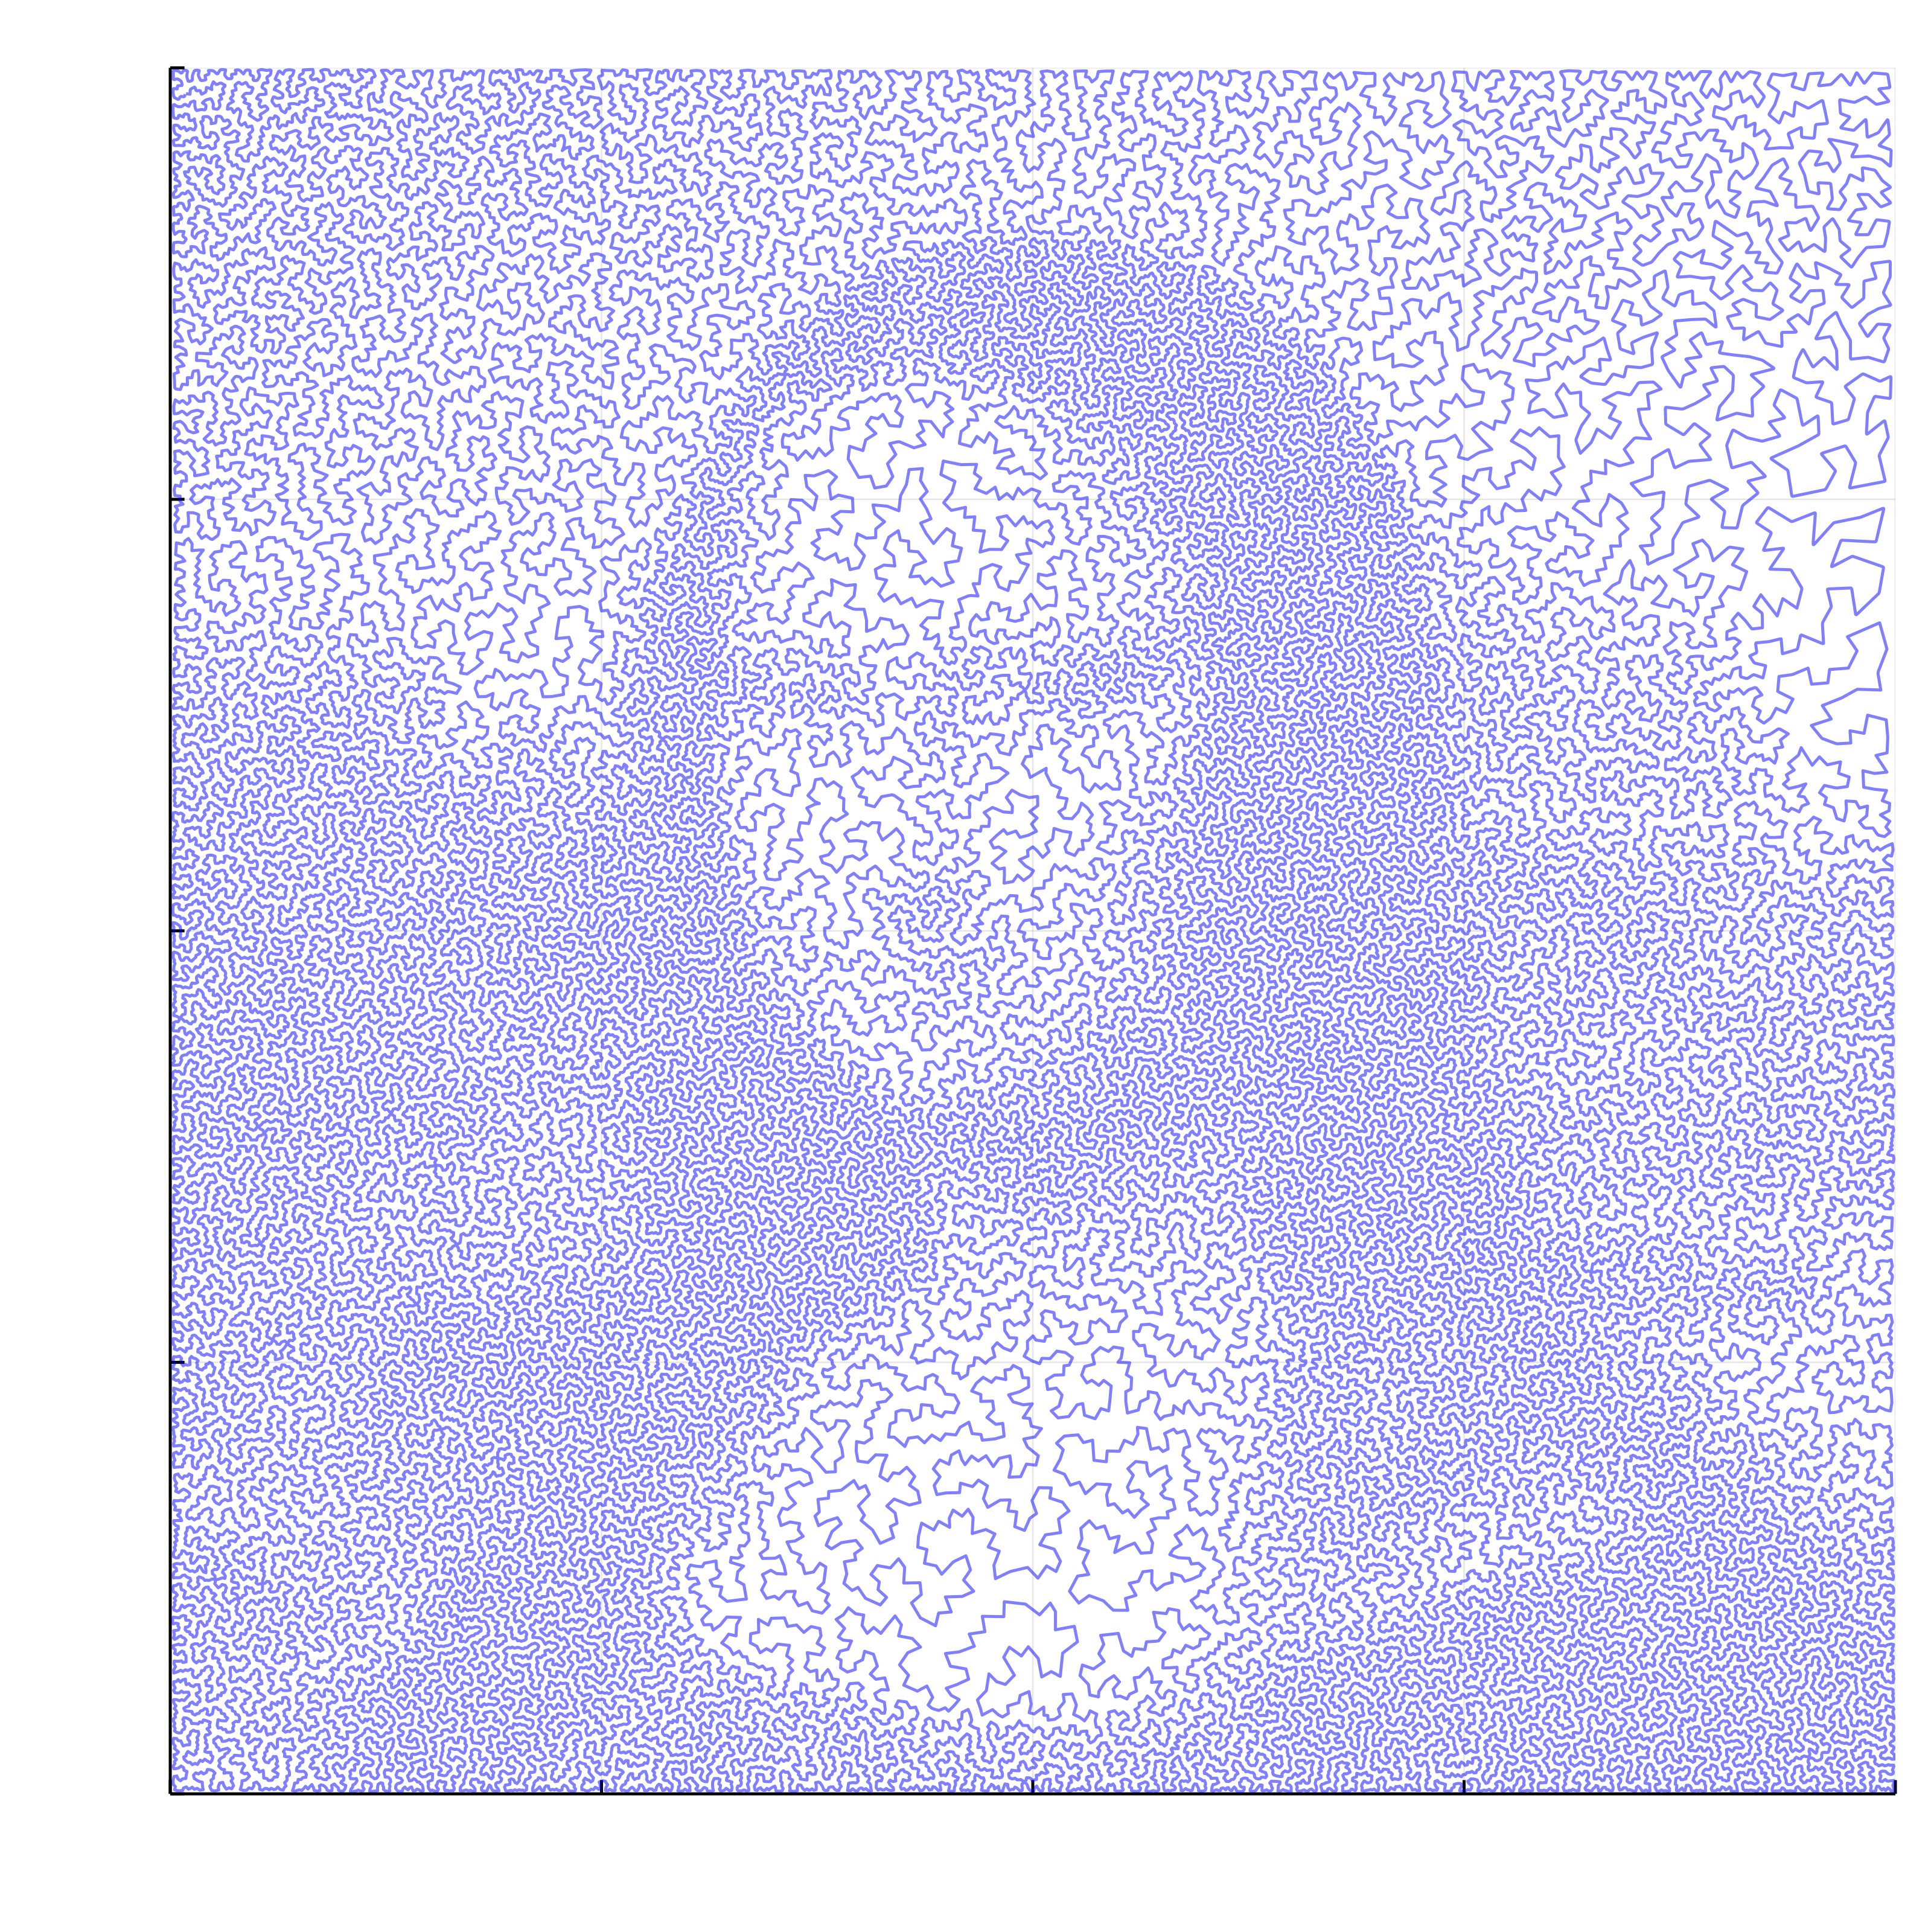
\includegraphics[width=\textwidth]{images/elastic_neighbourhood/fig_1}
	\def\c{Solution for the Mona Lisa art tour generated in 31 minutes using the bootstrapped Elastic Neighbourhood algorithm. }
	\caption[\c]{\label{fig:monalisa} \c The error of the computed solution is within a fraction of 0.07 of the known best tour calculated using 114 hours of supercomputer time with EAX-GA. Truncating the EAX-GA search at the 30 minute mark would result in a tour of over double the length of optimal and it would take EAX-GA approximately 30 hours to surpass the 0.07 fractional error barrier \cite{Honda2013-ri}.}
\end{figure}
Solutions are computed for each of the art tours in the dataset and compared to best known solutions, all of which were computed by EAX-GA \cite{Nagata2013-we}. These results are shown in Table \ref{table:art} and the images from solved instances are shown in Appendix B. The quality gap notably does not decrease with the increasing length but the performance when measured as a function of time does. This indicates, as does the theoretical bound, that these tours have been solve to near-optimality.
\begin{table}
	\centering
	\begin{tabular}[width=0.75\textwidth]{| c||  c | c |c | c | c|}
		\hline
		Tour& Num. Nodes & \makecell{Relative Tour \\ Length} & \makecell{E. Neigh. \\ Time (Hours)} &  \makecell{EAX-GA \\ Time (Hours)} & Speed-Up\\
		\hline
		Mona Lisa & $1\times10^5$ & 1.072 & 0.52 & 114.4 & 0.00451\\
		Van Gogh & $1.2\times10^5$ & 1.068 & 0.74 & 179.1& 0.00415 \\
		Venus & $1.4\times10^5$  &1.068 & 1.01 & 254.1 & 0.00398\\
		Pareja & $1.6\times10^5$& 1.070 & 1.32 & 409.4 & 0.00322\\
		Courbet  &$1.8\times10^5$ & 1.071 & 1.67 & 486.4 & 0.00343\\
		Earring & $2\times10^5$ & 1.075 & 2.06 & 676.0 & 0.00305 \\
		\hline
	\end{tabular}
	\def\c{Performance and timing results (hours) against the best-in-class EAX-GA solver for the Art TSP data set. }
	\caption[\c]{\label{table:art} \c The nodes in each tour range from $1 \times 10^5$ to $ 2 \times 10^5$ in steps of $20000$. The tour length errors are relatively constant at approximately 7\%. The timing scales approximately linearly with an additional 20000 nodes increasing convergence time by approximately 15 minutes which is substantially better than in both absolute time and complexity scaling. The scaling benefits are highlighted by the speed-up which increases from 200 to 300 fold as the tour sizes increase. The computational speed up in conjunction with the reliable error highlight the benefits of the Elastic Neighbourhood as a heuristic.}
\end{table}

\subsection{Feature Selectivity}
The Elastic Net offered an explanation on the formation of orientation maps in cortical space and made the prediction that the retinotopic projection would be distorted as a result of clustering the features concurrently \cite{Durbin1990-tn}. This retinotopic distortion has not had conclusive biological evidence to substantiate it. 
\begin{figure}
	\begin{subfigure}{0.5\textwidth}
		\centering
		\includegraphics[width=\textwidth]{images/introduction/distortedretinotopy}
		\caption{}
	\end{subfigure}
	\begin{subfigure}{0.4\textwidth}
		\centering
		\includegraphics[width=\textwidth]{images/introduction/V1retinotopy}
		\caption{}
	\end{subfigure}
	\caption{The distorted retinotopic projection predicted by the Elastic Net model is shown in panel (a).  Trained retinotopic locations are given by the intersection of the grid and the size of the black squares indicates the rate of change of the orientation variable. Distorted retinotopic fields are generated around regions where the orientation selectivity changes most rapidly. Optical imaging scans in both azimuthal and elevational of two phenotypes of regular (B) and deficient (C) spontaneous activity patterns are shown in panel (b). In both instances the phase and bulk activity scans do not show a distorted retinotopic map. Image reproduced from \cite{Cang2005-eg}. }
\end{figure}
Feature selectivity is examined by encoding a set of vectors with three components $\vec{y} = (y_1,y_2,y_3)$ using the Elastic Neighbourhood procedure. The cortical indices are encoded on a grid of 40x40 cells and stimulus batches with 400 nodes randomly distributed in the intervals [0,1], [0,1], and [0,0.1] are presented which in line with the original study. The minimisation is performed using the ADAM optimiser for 100 time steps at $dt = 0.01$, $K = 0.05$, $\alpha = 1$, $\beta = 0.001$ and $\gamma = 0.025$ for competition and $\gamma = 0$ for no competitive interaction. These parameters mimic those used in the original study, but the optimisation procedure is different. The net is evolved by presenting 5 batches of stimuli and measuring the resulting cortical map and retinotopy for a competition and competition-free system. These results are shown in Figure \ref{fig:endistortedretinotopy}. The competition-free results demonstrate that the ADAM minimisation can replicate the principle results of the original study. Adding competition demonstrates that cortical feature maps are still generated while preserving a distortion free retinotopy.
\begin{figure}
	\begin{subfigure}{0.5\textwidth}
		\centering
		\includegraphics[width=\textwidth]{images/elastic_neighbourhood/fig_elastic_net_feature}
		\caption{}
	\end{subfigure}
	\begin{subfigure}{0.5\textwidth}
		\centering
		\includegraphics[width=\textwidth]{images/elastic_neighbourhood/fig_elastic_net_retinotopy}
		\caption{}
	\end{subfigure}
	\begin{subfigure}{0.5\textwidth}
		\centering
		\includegraphics[width=\textwidth]{images/elastic_neighbourhood/fig_elastic_neighbourhood_feature}
		\caption{}
	\end{subfigure}
	\begin{subfigure}{0.5\textwidth}
		\centering
		\includegraphics[width=\textwidth]{images/elastic_neighbourhood/fig_elastic_neighbourhood_retinotopy}
		\caption{}
	\end{subfigure}
	\def\c{The cortical feature and retinotopic maps generated in a competition free and competitive environments are presented.}
	\caption[\c]{\label{fig:endistortedretinotopy} The cortical feature map generated in a competition free environment is presented in panel (a) and the distorted retinotopic map is presented in panel (b). These maps are consistent with the Elastic Net using Gauss-Seidel for minimisation. The cortical feature map with competitive interactions is shown in panel (c) with the associated retinotopic grid shown in panel (d). The feature map remains qualitatively similar to that generated by the Elastic Net but there is a smoother retinotopic coverage which is consistent with biological data.}
\end{figure}
The retinotopic projection generated by the Elastic Neighbourhood appears to be more uniformly distributed than the Elastic Net. This is quantified by partitioning cortical space into a grid and calculating a simple $\chi^2$ statistic under the assumption that points within each grid partition are distributed uniformly. Figure \ref{fig:chi2statistics} shows this measure of uniformity for the Elastic Neighbourhood, the Elastic Net, and a sample of uniformly distributed points.

\begin{figure}
	\centering
	\includegraphics[width=\textwidth]{images/elastic_neighbourhood/fig_chi2_statistics_uniform}
	\def\c{A measure of uniformity of the Elastic Net and Neighbourhood compared with a sample of uniformly distributed points. }
	\caption[\c]{\label{fig:chi2statistics} \c For each grid resolution the space is divided into $n\times n$ blocks and each of these forms an observation in the $\chi^2$ statistic with the expected number of points being $N/n^2$ where $N$ is the number of beads in the net. The Elastic Neighbourhood is quantifiably more uniform than the Elastic Net under this measure approaching what is expected for a sample of uniformly distributed points. It manages to maintain this uniformity in conjunction with developing a feature selective map that is at least as rich as the original Elastic Net algorithm.}
\end{figure}

\newpage
\section{Discussion}
The Elastic Net model has been extended by incorporating a competitive mechanism. This competitive mechanism improves on the biological explanatory power of the Elastic Net. The competitive mechanism also introduces desirable mathematical qualities which improve on the performance of the Elastic Net as a TSP heuristic. Several key aspects of the results will be discussed: feature selectivity, heuristic performance, scaling laws, the wire-minimisation problem, and potential future work.
\paragraph{Feature Selectivity} 
Feature selectivity was examined by augmenting the bead and node vectors to be 3-dimensional; this might, for example, correspond to an encoding of position and orientation values in the receptive field. The minimisation procedure was applied on the energy functional for a series of presentations of stimulus by sampling nodes with specific receptive field properties: this would correspond to the spontaneous waves of activity seen in early development \cite{Meister1991-mu, Burbridge2014-ib}. These stimuli were presented in batches and the minimisation problem solved on each batch. 

The results show that both a competitive and non-competitive environment results in clustering of features. In the positional vectors this corresponds to retinotopy. The non-competitive environment distorts these features quite dramatically with many receptive fields collapsing to single lines rather than being defined by a cortical volume. This replicates the result first shown by Durbin and Mitchison (1990) and the effect became even more pronounced with larger batch sizes \cite{Durbin1990-tn}. The competitive environment did not have as pronounced a distortion effect and this can be seen as a result of the space filling properties introduced by competition. This is particularly crucial in the case of positional features because a distortion in the retinotopy would result in a biological organism finding it challenging to scan a visual scene without compensatory mechanisms. Furthermore, these visual distortions have not been measured in functional imaging scans of mice superior colliculus maps which have been shown to have orientation preference \cite{Cang2005-eg, Feinberg2015-eu}. 

It is notable that the Elastic Neighbourhood method produces a feature map that is at least as rich as that of the Elastic Net. This suggests that there is no trade-off for retinotopic uniformity and offers an explanation why there is no notable observed retinotopic distortions in feature maps. Competitive mechanisms, in this context, act as a mechanism to preserve stereotypical and reliable anatomical development while allowing for rich stimulus specific learning.
\paragraph{TSP Heuristic Performance}
A number of studies to examine the Elastic Neighbourhoods performance as a TSP heuristic were conducted. In the first instance, the Elastic Neighbourhood was compared to the Elastic Net by initialising the algorithm at the centre of mass of the nodes. The introduction of competition allows it to outperform the Elastic Net particularly as tours get larger as shown in Figure \ref{fig:elasticneighbourhoodvsnet}. This can be attributed to the first property conferred by the competitive mechanism: tours are penalised for crossing over. In the original Elastic Net algorithm cross-overs were prevented by a slow annealing schedule which adds to the runtime and potentially gave the energy functional some property which made low energy tours difficult to find.

The initialisation position was allowed to vary and a series of meta-optimisation experiments on this initial position were performed for a small tour with 250 nodes. An initial grid search showed that for both uniformly distributed and skew-distributed data there are hotspots of high and low performance. There is no obvious pattern or structure to these hotspots and implying that it is just the specifics of the tour which define them. The meta-heuristics applied were random sampling, simulated annealing, and particle swarm optimisation. The random sampling method was not particularly performant. Simulated annealing and particle swarm before followed an exponential decay curve starting from an average relative error of approximately $0.08$ and levelling out to an error of about $0.025$ in 100 and 25 trials respectively. However, Particle Swarm optimisation takes more calls and so the performance-run time trade-off is comparable. These studies suggest that the algorithm can be improved by meta-optimisation.

The Elastic Neighbourhood was finally compared to two state of the art TSP heuristics: EAX-GA and LKH. The Elastic Neighbourhood was initialised with a fractal generator and completed 25 samples of tours ranging from 10000 to 30000 nodes. These are considered reasonably challenging with recommended run-times of several hours for both EAX-GA and LKH. The time-constrained and time-unconstrained cases were examined showing the Elastic Neighbourhood tends to outperform these heuristics in speed while still generating acceptable quality solutions in the ~7.5\% range and this performance gap increases with increasing node number. When time-cost is not a requirement to be minimised both EAX-GA and LKH become more performant which is to be expected because they will asymptotically search the entire solution space. The performance of the Elastic Neighbourhood has almost no dependence on length. This suggests it is a good heuristic for generating a tour with an almost certain convergence time and error bound which is are two highly desirable features. It also suggests that the performance is limited and cannot generate high quality tours which is undesirable when precision is more important than time-cost.
\paragraph{Scaling}
As seen in Figure \ref{fig:heuristicsperformance} and discussed previously the Elastic Neighbourhood appears to have no length dependence on solution quality. At least in randomly distributed tours of $N$ nodes it will converge to approximately 0.765$\sqrt{N}$ in all instances. This can be attributed to the space filling nature of the competitive mechanism which is demonstrated in Figure \ref{fig:selffillingcurve}. It seems likely that the algorithm is finding solutions which distribute the beads of the net in a fashion corresponding to some inbuilt fractal dimension of the algorithm. A point of future research would be to examine if this scaling constant can be manipulated because any improvement would immediately apply to large tour instances.

 There are two clear directions in which this line of research can proceed: parameter manipulation and initialisation. Tours are bootstrapped with a fractal and so this property may be a feature of the initialisation. This is unlikely because the scaling result extends to very non-uniform tours in the art data set which implies that it is a result of the competition interacting with the Laplacian and the geometry. It may, however, effect the performance which can be seen in the meta-optimisation studies. The first point of future research would be to examine fractal curves other than MPeano to see if they improve performance; this will be most fruitful in tours which have dramatically different structure to a random collection of points. The second way  the scaling factor can be improved is by parameter manipulation. No tuning was performed on this scaling constant with parameters chosen largely on force based arguments and previous research. However, initial exploratory experiments revealed that careful selection of the competition scaling parameter $\gamma$ could result in a $\beta_s$ closer to $0.746$ and a constant scaling of competition rather than annealing it with $K$ resulted in performant but non-convergent tours achieving a $0.05$ error bound on the Mona-Lisa. These experiments are the natural starting point to examine the scaling properties.
\paragraph{Wire-minimisation}
The neural wire-minimisation hypothesis is that a collection of neurons will instantiate connections on the basis of two constraints: functional computation and minimal wiring \cite{Koulakov2001-je}. The systems circuit must be able to perform the relative computations and after this condition has been satisfied an efficient wiring carries a metabolic and therefore fitness advantage and will be genetically selected \cite{Koulakov2004-ia}. This is a \textit{post-hoc} hypothesis that enjoys credibility from observed data \cite{Bartha2019-ve, Vertes2012-uv}. The Elastic Net served as a good conceptual model which demonstrated a mechanistic explanation for why near-optimal wiring in neural systems is expected without \textit{a priori} intensive genetic coding. A duality between the Elastic Net and the Kohonen model was argued for and this result is not surprising given they share a root concept introduced by the Tea Trade model \cite{Mitchison1995-cb, Kohonen1990-ys, Willshaw1976-ew} The natural Hebbian learning mechanisms found in the brain can generate the computational and wiring requirements \textit{de novo} \cite{Durbin1990-tn, Swindale2001-gh}. 

The Elastic Neighbourhood model introduced here extends this concept by adding biological plausibility and performance and makes a key prediction. The principle result is that competition is a natural part of a large corpus of biological systems and its inclusion substantially improves performance on the abstract wire minimisation task: the TSP. This substantiates the Elastic Net model as a principle mechanistic explanation of wire brains are wired so efficiently. Adding the competitive aspect improves the hypothesis by allowing a regular structure to emerge in feature space which is not just homeomorphic to the existing retinotopic map but is largely bijective with it. This is a desirable feature when biological systems have to align multiple areas of computation with the principle data which is retinotopically organised \cite{Savier2017-wt}. Finally, adding competitive makes the minimisation procedure robust: it reliably converges to a wiring volume which is consistent at every scale. Reliable development which does not have to be genetically hard-coded is extremely valuable: it allows for improved genetic fitness as the genome may be more efficiently coded, can be conserved across multiple organisms, and allows for efficient calibration with other mechanisms which are implicated in the correct functioning of a system but are tangentially related.

\paragraph{Limitations}
This study is limited by overall performance: there appears to be a constraint that forces the error in the solution to a constant value of ~8\% in the uniformly distributed cases and 7\% in the art distributions. This error can be improved by apply a meta-heuristic optimisation in addition to the Elastic Neighbourhood but this would likely nullify the time performance benefits gained by the model. The LKH and EAX-GA heuristics find a near-optimal solution given enough time and this limits the use of the Elastic Neighbourhood to situations where time constraints outweigh the benefits of a shorter tour. The convergence to a constant error would be useful in making this assessment as the performance is known, at least approximately, \textit{a priori}.

The model of feature selectivity is limited by specificity: it is too abstract in its current form to make concrete testable predictions. It notably diverges from the Elastic Net in the prediction of distorted retinotopy but does not substantiate the conceptual arguments made about feature selectivity and wire-minimisation. The mouse superior colliculus does not appear to have appreciably distorted retinotopy and has recently been observed to have orientation preferences \cite{Feinberg2014-mj}. These observations would be a natural first line of future research.

\paragraph{Future Work}
As a heuristic there are three lines of immediate pursuit. The scaling constant of the model may be improved by parameter tuning and careful examinations of the initialisation schemes. Any reduction in this scaling constant would immediately propagate with no computational cost. Further technical enhancements can be made so that it is efficiently implemented as a software routine.

As a biological model two properties can be immediately investigated: feature map prediction and wire-length prediction. There are an increasing number of high resolution cortical feature maps being generated \cite{Bednar2016-lg}. A useful model system is the mouse retinotopic map in the superior colliculus which is relatively undistorted and demonstrates orientation preferences \cite{Feinberg2014-mj}. By calibrating the Elastic Neighbourhood against these relative energy contribution of competition and activity can be gauged. By understanding this ratio predictions can be made about the total cortical wiring length which presents a falsifiable hypothesis. This work would likely need to be more rigorously grounded in its mechanisms: it is currently too abstract to be falsifiable. A useful starting point in this regard could be the Distributed Kernels model proposed in the previous chapter as it can currently explain many aspects of the simpler retinotopic mapping.

\paragraph{Key Summary}
\begin{enumerate}
	\item \textit{The Elastic Net has been extended to include competitive interactions between the beads and to use the ADAM optimiser: the Elastic Neighbourhood. These inclusions have been implemented using highly parallelised GPU code leading to substantial performance benefits in both performance and execution time.}
	\item \textit{As a TSP heuristic the Elastic Neighbourhood has good performance. It is comparable or favourable to the state of the art solvers EAX-GA and LKH when these are time-limited to similar execution times.}
	\item \textit{The solution error in the Elastic Neighbourhood converges to an approximate constant. This is useful for confidently assessing the costs of lost time against potential improvements on solution correctness. The convergence to constant error is observed even in large datasets with $>100000$ nodes such as those found in the Art TSP database. These large tours typically require hundreds of hours of compute resources while the Elastic Neighbourhood executes in hours.}
	\item \textit{The Elastic Neighbourhood was examined in the context of feature selectivity and was found to be capable of generating feature maps while maintaining relatively undistorted underlying retinotopy.}
\end{enumerate}